\ifdefined\ishandout
\documentclass[handout]{beamer}
\else
\documentclass{beamer}
\fi

\usepackage[frenchb]{babel}
\usepackage[T1]{fontenc}
\usepackage[latin1]{inputenc}
\usepackage{hyperref}
\usepackage{multirow}
\usepackage{listings}
\usepackage{fancyvrb}
\usepackage{tikz}
\usepackage{framed}
\usepackage{algorithm}
\usepackage{algorithmic}
\usepackage{xcolor}
\usepackage{color, colortbl}
\usepackage{handoutWithNotes}

\usetikzlibrary{shapes.geometric}
\usetikzlibrary{positioning}
\usetikzlibrary{shapes.arrows, chains}
\usetikzlibrary{arrows,calc}
\usepackage{array}
\usetheme{Boadilla}

\ifdefined\ishandout
\pgfpagesuselayout{3 on 1 with notes}[a4paper,border shrink=5mm]
\usecolortheme{dove}
\else
\usecolortheme{dolphin}
\fi


\lstnewenvironment{codeC}
{ \lstset{language=C,
    otherkeywords={printf,scanf}}
}
{}

\ifdefined\ishandout
\definecolor{mygreen}{rgb}{0,0,0}
\definecolor{mymauve}{rgb}{0,0,0}
\definecolor{myblue}{rgb}{0,0,0}
\else
\definecolor{mygreen}{rgb}{0,0.6,0}
\definecolor{mymauve}{rgb}{0.58,0,0.82}
\definecolor{myblue}{rgb}{0,0,1}

\fi

\definecolor{mygray}{rgb}{0.5,0.5,0.5}


\lstset{language=C,
% breakatwhitespace=false,         % sets if automatic breaks should only happen at whitespace
%  breaklines=true,                 % sets automatic line breaking
%  captionpos=b,                
commentstyle=\itshape\color{mymauve},
keywordstyle=\bfseries\color{myblue},
%numbers=left,                    % where to put the line-numbers; possible values are (none, left, right)
%  numbersep=8pt,                   % how far the line-numbers are from the code
%  numberstyle=\tiny\color{mygray}, % the style that is used for the line-numbers
  rulecolor=\color{black},         % if not set, the frame-color may be changed on line-breaks within not-black text (e.g. comments (green here))
%  showspaces=false,                % show spaces everywhere adding particular underscores; it overrides 'showstringspaces'
  showstringspaces=false,          % underline spaces within strings only
%  showtabs=false,                  % show tabs within strings adding particular underscores
%  stepnumber=2,                    % the step between two line-numbers. If it's 1, each line will be numbered
  stringstyle=\color{mygreen},     % string literal style
%  tabsize=2 
}

\newcommand{\red}{\textcolor{red}}
%\newcommand \emph
%Default size : 12.8 cm * 9.6 cm

\newcommand{\tmark}[1]{\tikz[remember picture, baseline=-.5ex]{\coordinate(#1)}}

\ifdefined\ishandout
\newenvironment<>{codeblock}[1]{%begin
  \setbeamercolor{block title}{fg=black,bg=lightgray!80}%
  \begin{block}{#1}}
  % \begin{codeC}}
  %  {\end{codeC}
{  
\end{block}}

\newenvironment<>{termblock}[1]{
    \setbeamercolor{block title}{fg=black,bg=lightgray!90}%
    \begin{block}{#1}
}
%     \begin{Verbatim}}
{%\end{Verbatim}
\end{block}
}

\definecolor{bluegreen}{RGB}{0,0,0}
%\definecolor{bluegreen}{rgb}{0,0.6,0.8}
\else

\newenvironment<>{codeblock}[1]{%begin
  \setbeamercolor{block title}{fg=darkgray,bg=yellow}%
  \begin{block}{#1}}
  % \begin{codeC}}
  %  {\end{codeC}
{  
\end{block}}

\newenvironment<>{termblock}[1]{
    \setbeamercolor{block title}{fg=white,bg=lightgray}%
    \begin{block}{#1}}
%     \begin{Verbatim}}
{%\end{Verbatim}
\end{block}
}

\definecolor{bluegreen}{RGB}{0,149,182}
%\definecolor{bluegreen}{rgb}{0,0.6,0.8}
\fi

%\newcommand{\output}[1]{
\setbeamertemplate{navigation symbols}{}
\newcommand{\bvrb}{\Verb[commandchars=���,formatcom=\color{bluegreen}]}
\newcommand{\footvrb}{\footnotesize\Verb}


%%% Param�tres du cours (� r�gler)
%Num�ro du cours
\newcommand{\nb}{5}

\title[Cours n�\nb]{Cours n�\nb - Les Pointeurs (et les cha�nes de carat�res)}
\author[]{julien.brajard@upmc.fr}
\institute[Polytech' UPMC]{Polytech' UPMC}
\date{02 Novembre 2015}
\begin{document}
%%%%%%%%%%%%%%%%%%%%% SLIDES DE TITRE
\begin{frame}
\titlepage
\centering{
\url{http://australe.upmc.fr} (onglet EPU-C5-IGE Info Gen)}
\end{frame}
%%%%%%%%%%%%%%%%%%%%%
\begin{frame}
\frametitle{Plan du cours n�\nb}
\tableofcontents[hideallsubsections]
\end{frame}

%%%%



%%%%%% SECTION 12
% !TEX encoding = IsoLatin9

%%%%%%%%%%%%%%%%%%%%% SECTION 1
\section{Les cha�nes de caract�res}
\begin{frame}
  \begin{columns}
    \column{4.8cm}
    \tableofcontents[currentsection,hideothersubsections]
    \column{7cm}
    
  \end{columns}
  
\end{frame}

\begin{frame}[fragile]
\frametitle{Les cha�nes de caract�res}
\begin{itemize}
\setlength\itemsep{1em}
\item Les cha�nes de carat�res sont des tableaux
de caract�res ;
\item Chaque case du tableau contient un caract�re ;
\item Le dernier �l�ment est \red{toujours} \Verb|'\0'| ;
\item Pour socker une cha�ne de \Verb|n| �l�ments, il
faut \Verb|n+1| emplacements (� cause du \Verb|'\0'|).
\end{itemize}

\end{frame}

\begin{frame}[fragile]
\frametitle{Initialisation des cha�nes de carat�res}
\begin{block}{}
On peut utiliser les doubles quotes \Verb|"| pour initialiser
une cha�ne de caract�res.
\end{block}

\begin{codeblock}{}
\vspace{-.3cm}
\lstset{escapeinside={��}}
\lstset{basicstyle=\scriptsize}
\begin{codeC}
char tab[] = {'i','n','f','o','r','m','a','t','i','q','u','e','\0'};
\end{codeC}
\vspace{-.3cm}
\end{codeblock}
\vspace{1em}
\centering {ou}
\vspace{1em}
\begin{codeblock}{}
\vspace{-.3cm}
\lstset{escapeinside={��}}
\lstset{basicstyle=\scriptsize}
\begin{codeC}
char tab[] = "informatique";
\end{codeC}
\vspace{-.3cm}
\end{codeblock}
\end{frame}

\begin{frame}[fragile]
\frametitle{Le \bvrb|printf| et les cha�nes de caract�res}

\begin{block}{}
Le formateur de la cha�ne de caract�res dans le \bvrb|printf|
est \bvrb|%s|.
\end{block}
\vspace{1em}

Exemple :
\begin{codeblock}{}
\vspace{-.3cm}
\lstset{escapeinside={��}}
\lstset{basicstyle=\scriptsize}
\begin{codeC}
char tab[] = "informatique";
printf("Nous sommes en cours d'%s\n",tab);
\end{codeC}
\vspace{-.3cm}
\end{codeblock}
\end{frame}

\begin{frame}[fragile]
\frametitle{Saisie de cha�nes de carat�res au clavier}
Il existe deux fonctions en langage C permettant
de saisir des cha�nes de caract�res :
\begin{itemize}
\setlength\itemsep{1em}
\item \bvrb|scanf| (d�j� vu) ;
\item \bvrb|fgets| (sp�cifique pour les cha�nes de caract�res).
\end{itemize}
\end{frame}

\begin{frame}[fragile]
\frametitle{Les \bvrb|scanf| et les cha�nes de caract�res}
\begin{itemize}
\setlength\itemsep{1em}
\item Le formateur de la cha�ne de caract�re dans le
\bvrb|scanf| est \bvrb|%s|.
\item Pensez � d�clarer un tableau de caract�res d'une
taille suffisante avant de l'affecter dans le \bvrb|scanf|.
\item Il ne faut \red{pas} mettre le \bvrb|&|.
\end{itemize}
\begin{codeblock}{}
\vspace{-.3cm}
\lstset{escapeinside={��}}
%\lstset{basicstyle=\scriptsize}
\begin{codeC}
char nom[20];
printf("\n Entrez votre nom : ");
scanf("%s",nom);
printf("\n Bonjour %s !\n",nom);
\end{codeC}
\vspace{-.3cm}
\end{codeblock}

\end{frame}

\begin{frame}[fragile]
\frametitle{Rappel : le caract�re espace}

\begin{block}{}
Le caract�re espace est consid�r� comme un d�limiteur.
La conversion de la m�moire tampon en cha�ne de caract�res
s'arr�te donc � l'espace et ce dernier n'est pas consomm� :
il reste disponible pour la prochaine lecture.
\end{block}

\begin{columns}

\column{0.49\textwidth}

\begin{codeblock}{exemple.c}
\vspace{-.3cm}
\lstset{escapeinside={��}}
\lstset{basicstyle=\scriptsize}
\begin{codeC}
char nom[20];
printf("\n Entrez votre nom : ");
scanf("%s",nom);
printf("\n Bonjour %s !\n",nom);
\end{codeC}
\vspace{-.3cm}
\end{codeblock}

\column{0.45\textwidth}

\begin{termblock}{test 1}
\vspace{-.3cm}
\lstset{escapeinside={��}}
\lstset{basicstyle=\scriptsize}
\begin{lstlisting}
�\textbf{>>}�./exemple
�\color{darkgray}{\texttt{Entrez votre nom : }}� Dupont
�\color{darkgray}{\texttt{Bonjour Dupont ! }}�
\end{lstlisting}
\vspace{-.3cm}
\end{termblock}

\begin{termblock}{test 2}
\vspace{-.3cm}
\lstset{escapeinside={��}}
\lstset{basicstyle=\scriptsize}
\begin{lstlisting}
�\textbf{>>}�./exemple
�\color{darkgray}{\texttt{Entrez votre nom : }}� Dupont toto
�\color{darkgray}{\texttt{Bonjour Dupont ! }}�
\end{lstlisting}
\vspace{-.3cm}
\end{termblock}

\end{columns}
\begin{alertblock}{Conclusion}
Avec \bvrb|scanf| on ne peut pas saisir de cha�ne
de caract�res avec des espaces.
\end{alertblock}

\end{frame}

\begin{frame}[fragile]
\frametitle{Autre solution : \bvrb|fgets|}
\centering{
  \bvrb|fgets(�textit�string�,�textit�taille�,stdin);|
}
\begin{columns}

\column{0.49\textwidth}

\begin{codeblock}{exemple.c}
\vspace{-.3cm}
\lstset{escapeinside={��}}
\lstset{basicstyle=\scriptsize}
\begin{codeC}
char nom[20];
printf("\n Entrez votre nom : ");
fgets (nom,19,stdin) ;
printf("\n Bonjour %s !\n",nom);
\end{codeC}
\vspace{-.3cm}
\end{codeblock}

\column{0.45\textwidth}

\begin{termblock}{test}
\vspace{-.3cm}
\lstset{escapeinside={��}}
\lstset{basicstyle=\scriptsize}
\begin{lstlisting}
�\textbf{>>}�./exemple
�\color{darkgray}{\texttt{Entrez votre nom : }}� Dupont toto
�\color{darkgray}{\texttt{Bonjour Dupont toto ! }}�
\end{lstlisting}
\vspace{-.3cm}
\end{termblock}
\end{columns}

\begin{itemize}
\item Avec \bvrb|fgets|, seule la fin de ligne sert de d�limiteur.
\item \bvrb|�textit�taille�| est le nombre maximum de caract�res
qui peuvent �tre lus.
\item \bvrb|stdin| indique qu'on doit lire les caract�res
dans "l'entr�e standard", c'est � dire dans ce que vous tapez
au clavier. On peut aussi lire les caract�res dans un fichier
(cf cours n$^o$ 7)
\item \red{ATTENTION} : la cha�ne de caract�re lue contiendra le
retour � la ligne.
Dans l'exemple pr�c�dent 
\Verb|nom='D','u','p','o','n','t',' ','t','o','t','o','\n','\0'|
\end{itemize}

\end{frame}

\begin{frame}
\frametitle{�galit� de cha�nes de caract�res}
\begin{block}{}
Pour v�rifier l'�galit� de deux cha�nes de caract�res,
il faut v�rifier un par un tous les caract�res (comme
pour un autre tableau).
\end{block}

\vspace{1em}
\begin{exampleblock}{Exemple :}

Demander � l'utilisateur d'entrer \Verb|pluie| ou \Verb|soleil|,
et afficher "Prenez un parapluie" si l'utilisateur � mis pluie.
\end{exampleblock}
\end{frame}

\begin{frame}[fragile]
\frametitle{La biblioth�que \bvrb|string.h|}
\begin{codeblock}{exemple.c}
\vspace{-.3cm}
\lstset{escapeinside={��}}
%\lstset{basicstyle=\scriptsize}
\begin{codeC}
#include <string.h>
\end{codeC}
\vspace{-.3cm}
\end{codeblock}

\begin{block}{}
Contient des fonctions standards pour g�rer les 
cha�nes de caract�res
\end{block}
Exemples :
\begin{figure}
\centering
\begin{tabular}{|c|p{3.8cm}|}
\hline
Prototype de la fonction & Utilisation \\
\hline
\bvrb|int strcmp(char �textit�s1�[], char �textit�s2�[]);| &
\red{Renvoie}  si les les cha�nes \bvrb|�textit�s1�| et \bvrb|�textit�s2�|
sont �gales.\\
\hline
\bvrb|int strlen(char �textit�s�[]);| & 
Renvoie la taille de \bvrb|�textit�s�|\\
\hline
\end{tabular}
\end{figure}

Pour le d�tail de toutes les fonctions :
\begin{termblock}{}
\vspace{-.3cm}
\lstset{escapeinside={��}}
%\lstset{basicstyle=\scriptsize}
\begin{lstlisting}
�\textbf{>>}� man string
\end{lstlisting}
\vspace{-.3cm}
\end{termblock}
\end{frame}
\end{document} 

%%%%%%%%%%%%%%%%%%%%% SECTION 1
\section{Les algorithmes}\label{section:1}
\begin{frame}
\begin{columns}
        \column{4.8cm}
            \tableofcontents[currentsection]
        \column{7cm}
        \centering{
            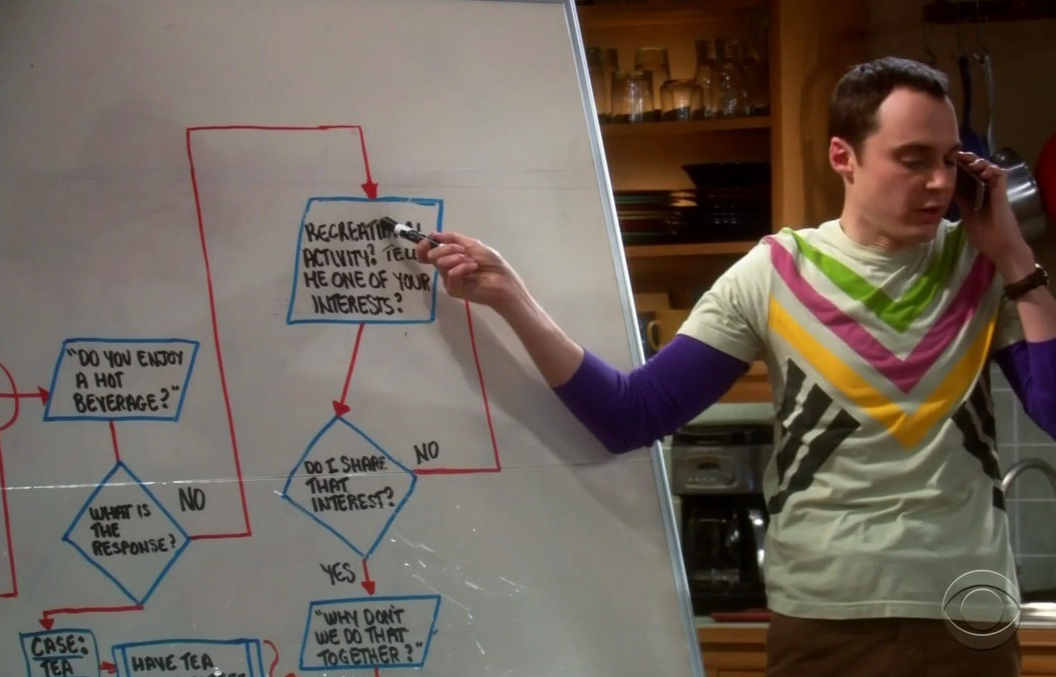
\includegraphics[width=7cm]{fig/Algorithm-sheldon.png}
            
                 \textit{ I believe I've isolateblblblblblblsblbslbslbsl
            sblbslblsblsblblsblbs
            lbslblbslsb d the algorithm for making friends.}
     
            
            \small{
            \hfill Sheldon Cooper, 
            
            \hfill in \textit{The Big Band Theory}, Season 2, Episode 13
            }
}

    \end{columns}

\end{frame}


%%%%%%%%%%%%%%%%%%%%%
\subsection{Introduction}
    \begin{frame}
    \frametitle{Pourquoi faire appel � des algorithmes ?}
    Pour automatiser des t�ches
    
    Exemples :
    \begin{itemize}
    \item M�tier � tisser\\
    \item M�thode de calcul � la main d'une division\\
    \item Recette de cuisine\\
    \item ...\\
    \end{itemize}
    \end{frame}
 
 %%%%%%%%%%%%%%%%%
 
    \begin{frame}
    \frametitle{Qu'est-ce qu'un algorithme ?}
    \begin{block}{D�finition}
    Un algorithme est un ensemble 
    ordonn� d'instructions simples
permettant de r�soudre un probl�me.
    \end{block}
    \end{frame}
    
 %%%%%%%%%%%%%%%%%%
 \subsection{Construction d'un algorithme}
%%%%%%%%%%%%%%%%%%%    
\section{La machine de Turing}
%%%%%%%%%%%%%%%%%%%%
 
  
\begin{frame}[fragile]
\frametitle{Un peu d'histoire...}
\begin{codeblock}{Test}
\begin{codeC}
for (int i = 0 ; i < n ; i ++) {
    //a comment
    printf("%d",i);
    }
\end{codeC}
\end{codeblock}

\begin{termblock}{test 2}
\lstset{escapeinside={��}}
\begin{lstlisting}
�\textbf{>>}�./a.out
�\color{darkgray}{\texttt{  Hello World}}�
\end{lstlisting}
\end{termblock}

 \begin{block}{Bloc standard}
blablabla
\end{block}
\end{frame}


\begin{frame}[fragile]
\frametitle{essai}
\begin{columns}
\column{6cm}
\begin{block}

\begin{figure}
\begin{tikzpicture} [
    auto,
    decision/.style = { diamond, draw=blue, thick, fill=blue!20,
                        text width=5em, text badly centered,
                        inner sep=1pt, rounded corners },
    block/.style    = { rectangle, draw=blue, thick, 
                        fill=blue!20, text width=10em, text centered,
                        rounded corners, minimum height=2em },
    line/.style     = { draw, thick, ->, shorten >=2pt },
  ]
   \matrix [column sep=-10mm, row sep=10mm] {
                    & \node [text centered] (x) {$\mathbf{X}$};            & \\
                    & \node (null1) {};                                    & \\
                    & \node [block] (doa) {\textsf{DoAE}($\mathbf{X}$)};   & \\
  	               \node(null3){}; & \node [decision] (uiddes)
                        {\textsf{UID}($\hat{\mathbf{X}}$)};
                                  & \node[text centered](tra){$\mathbf{i}$}; \\
                  & \node [block] (track) {\textsf{DoAT}($\mathbf{x}$)}; & \\
                    & \node [block] (pesos)
                        {\textsf{BF}(DoA$_{\mathrm{T}}$,DoAs)};            & \\
                    & \node [block] (filtrado)
                        {\textsf{SF}($\mathbf{w}$,$\mathbf{x}$)};          & \\
                    & \node [text centered] (xf) {$\hat{x}(t)$ };          & \\
  };
  % connect all nodes defined above
 \begin{scope} [every path/.style=line]
    \path (x)        --    (doa);
    \path (doa)      --    node [near start] {DoAs} (uiddes);
    \path (tra)      --    (uiddes);
    \path (uiddes)   --++  (-3,0) node [near start] {no} |- (null1);
    \path (uiddes)   --    node [near start] {DoA} (track);
    \path (track)    --    node [near start] {DoA$_{\mathrm{T}}$} (pesos);
    \path (pesos)    --    node [near start] {\textbf{w}} (filtrado);
    \path (filtrado) --    (xf);
  
  \end{scope}
\end{tikzpicture}
\end{figure}
\end{block}
\column{3cm}
\begin{block}{bulbul}
\end{block}
\end{columns}
\end{frame}

\end{document}
